% Options for packages loaded elsewhere
\PassOptionsToPackage{unicode}{hyperref}
\PassOptionsToPackage{hyphens}{url}
\PassOptionsToPackage{dvipsnames,svgnames,x11names}{xcolor}
%
\documentclass[
]{article}
\usepackage{amsmath,amssymb}
\usepackage{iftex}
\ifPDFTeX
  \usepackage[T1]{fontenc}
  \usepackage[utf8]{inputenc}
  \usepackage{textcomp} % provide euro and other symbols
\else % if luatex or xetex
  \usepackage{unicode-math} % this also loads fontspec
  \defaultfontfeatures{Scale=MatchLowercase}
  \defaultfontfeatures[\rmfamily]{Ligatures=TeX,Scale=1}
\fi
\usepackage{lmodern}
\ifPDFTeX\else
  % xetex/luatex font selection
\fi
% Use upquote if available, for straight quotes in verbatim environments
\IfFileExists{upquote.sty}{\usepackage{upquote}}{}
\IfFileExists{microtype.sty}{% use microtype if available
  \usepackage[]{microtype}
  \UseMicrotypeSet[protrusion]{basicmath} % disable protrusion for tt fonts
}{}
\makeatletter
\@ifundefined{KOMAClassName}{% if non-KOMA class
  \IfFileExists{parskip.sty}{%
    \usepackage{parskip}
  }{% else
    \setlength{\parindent}{0pt}
    \setlength{\parskip}{6pt plus 2pt minus 1pt}}
}{% if KOMA class
  \KOMAoptions{parskip=half}}
\makeatother
\usepackage{xcolor}
\usepackage[margin=1in]{geometry}
\usepackage{graphicx}
\makeatletter
\def\maxwidth{\ifdim\Gin@nat@width>\linewidth\linewidth\else\Gin@nat@width\fi}
\def\maxheight{\ifdim\Gin@nat@height>\textheight\textheight\else\Gin@nat@height\fi}
\makeatother
% Scale images if necessary, so that they will not overflow the page
% margins by default, and it is still possible to overwrite the defaults
% using explicit options in \includegraphics[width, height, ...]{}
\setkeys{Gin}{width=\maxwidth,height=\maxheight,keepaspectratio}
% Set default figure placement to htbp
\makeatletter
\def\fps@figure{htbp}
\makeatother
\setlength{\emergencystretch}{3em} % prevent overfull lines
\providecommand{\tightlist}{%
  \setlength{\itemsep}{0pt}\setlength{\parskip}{0pt}}
\setcounter{secnumdepth}{5}
\newlength{\cslhangindent}
\setlength{\cslhangindent}{1.5em}
\newlength{\csllabelwidth}
\setlength{\csllabelwidth}{3em}
\newlength{\cslentryspacingunit} % times entry-spacing
\setlength{\cslentryspacingunit}{\parskip}
\newenvironment{CSLReferences}[2] % #1 hanging-ident, #2 entry spacing
 {% don't indent paragraphs
  \setlength{\parindent}{0pt}
  % turn on hanging indent if param 1 is 1
  \ifodd #1
  \let\oldpar\par
  \def\par{\hangindent=\cslhangindent\oldpar}
  \fi
  % set entry spacing
  \setlength{\parskip}{#2\cslentryspacingunit}
 }%
 {}
\usepackage{calc}
\newcommand{\CSLBlock}[1]{#1\hfill\break}
\newcommand{\CSLLeftMargin}[1]{\parbox[t]{\csllabelwidth}{#1}}
\newcommand{\CSLRightInline}[1]{\parbox[t]{\linewidth - \csllabelwidth}{#1}\break}
\newcommand{\CSLIndent}[1]{\hspace{\cslhangindent}#1}
\ifLuaTeX
\usepackage[bidi=basic]{babel}
\else
\usepackage[bidi=default]{babel}
\fi
\babelprovide[main,import]{french}
% get rid of language-specific shorthands (see #6817):
\let\LanguageShortHands\languageshorthands
\def\languageshorthands#1{}
\usepackage{amsmath} \usepackage{geometry} \usepackage{pdfpages} \usepackage{fontspec} \usepackage{pdfpages} \usepackage{graphicx} \usepackage{amsmath} \usepackage{atbegshi} \usepackage{fancyhdr} \usepackage{tocloft} \usepackage{tcolorbox} \usepackage{xcolor} \definecolor{bleu}{RGB}{0,0,255} \usepackage{everypage} \usepackage{everypage} \usepackage{graphicx} \usepackage{fancyhdr} \pagestyle{fancy} \definecolor{mybrown}{RGB}{139,69,19} \fancyhead[R]{}
\usepackage{booktabs}
\usepackage{longtable}
\usepackage{array}
\usepackage{multirow}
\usepackage{wrapfig}
\usepackage{float}
\usepackage{colortbl}
\usepackage{pdflscape}
\usepackage{tabu}
\usepackage{threeparttable}
\usepackage{threeparttablex}
\usepackage[normalem]{ulem}
\usepackage{makecell}
\usepackage{xcolor}
\ifLuaTeX
  \usepackage{selnolig}  % disable illegal ligatures
\fi
\IfFileExists{bookmark.sty}{\usepackage{bookmark}}{\usepackage{hyperref}}
\IfFileExists{xurl.sty}{\usepackage{xurl}}{} % add URL line breaks if available
\urlstyle{same}
\hypersetup{
  pdflang={fr},
  colorlinks=true,
  linkcolor={Maroon},
  filecolor={Maroon},
  citecolor={Blue},
  urlcolor={blue},
  pdfcreator={LaTeX via pandoc}}

\author{}
\date{\vspace{-2.5em}}

\begin{document}

\setcounter{tocdepth}{5}                
\renewcommand\contentsname{\begin{center}\textcolor{brown}{Sommaire}\end{center}}
\AtBeginShipout{
  \ifnum\value{page}=1\thispagestyle{empty}\fi}
\pagestyle{fancy}
\fancyhf{}
\renewcommand{\headrulewidth}{0.4pt}
\renewcommand{\footrulewidth}{0.4pt}
\fancyhead[L]{Elèves Ingénieurs}
\fancyhead[R]{\textcolor{brown}{@Alex, Ali, Richard \& Toussaint}}
\fancyfoot[C]{\thepage}
\fancyfoot[L]{Mars 2025}
\fancyfoot[R]{Projet Statistique}
\AddEverypageHook{
  \ifnum\value{page}>1 
    \fancyhead[L]{Elèves Ingénieurs}
    \fancyhead[R]{\textcolor{brown}{@Alex, Ali, Richard \& Toussaint}}
    \fancyfoot[C]{\thepage}
    \fancyfoot[L]{Mars 2025}
    \fancyfoot[R]{Projet Statistique}
  \else
    \fancyhead[L]{} 
    \fancyhead[R]{}
    \fancyfoot[C]{}
    \fancyfoot[R]{}
  \fi
}

\tableofcontents

\newpage

\renewcommand\listtablename{\begin{center}\textcolor{brown}{Liste des Tableaux}\end{center}}
\renewcommand\listfigurename{\begin{center}\textcolor{brown}{Liste des Figures}\end{center}}

\setlength{\cftfignumwidth}{3em}
\setlength{\cfttabnumwidth}{3em}

\listoftables

\newpage

\listoffigures

\newpage

\hypertarget{introduction}{%
\section{Introduction}\label{introduction}}

La répartition géographique des besoins en soins de santé est un enjeu
majeur pour les politiques publiques, notamment en ce qui concerne
l'accès aux services de médecine de ville. Les inégalités territoriales
dans l'offre et la demande de soins peuvent entraîner des disparités
significatives en matière de santé, affectant particulièrement les
populations vivant dans des zones sous-dotées en professionnels de
santé. Comprendre ces dynamiques spatiales et socio-démographiques est
essentiel pour identifier les zones prioritaires et orienter les
décisions en matière d'allocation des ressources.

Dans ce contexte, ce travail propose une modélisation du nombre de
consultations en médecine de ville à l'échelle communale, en tenant
compte des caractéristiques démographiques, socio-économiques et
spatiales des communes. L'objectif est double : d'une part, analyser les
facteurs influençant la demande de soins, et d'autre part, identifier
les zones susceptibles de dépasser un seuil critique de ``désert
médical''. Pour ce faire, nous nous appuierons sur une base de données
riche et variée, comprenant des informations issues du Système National
des Données de Santé (SNDS) pour la période 2018-2022, ainsi que des
indicateurs socio-démographiques et géographiques.

Notre approche méthodologique repose sur une combinaison de techniques
statistiques et spatiales. Nous commencerons par une analyse descriptive
et cartographique des données pour visualiser les tendances et les
disparités territoriales. Ensuite, nous utiliserons des modèles de
régression de Poisson pour modéliser le nombre de consultations
annuelles, en tenant compte des effets fixes (caractéristiques des
communes) et des effets aléatoires (variations spatiales). Enfin, une
régression logistique binaire sera employée pour évaluer la probabilité
qu'une commune dépasse un seuil prédéfini de ``désert médical''.

Ce travail s'inscrit dans une perspective à la fois académique et
opérationnelle. Sur le plan académique, il contribue à l'étude des
inégalités territoriales en santé en proposant une méthodologie robuste
pour l'analyse spatiale des données de soins. Sur le plan opérationnel,
il fournit des outils pour identifier les zones prioritaires et soutenir
la prise de décision en matière de politiques de santé publique.

\hypertarget{pruxe9sentation-du-contexte}{%
\section{Présentation du contexte}\label{pruxe9sentation-du-contexte}}

\hypertarget{cadre-conceptuel-de-luxe9tude}{%
\subsection{Cadre conceptuel de
l'étude}\label{cadre-conceptuel-de-luxe9tude}}

Dans cette partie, nous allons définir certainses notions clés qui
apparaissent dans notre étude : le taux de visite et la notion de
voisin.

\hypertarget{taux-de-visite}{%
\subsubsection{Taux de visite}\label{taux-de-visite}}

Le taux de visite n'est rien d'autre que le nombre moyen de visite dans
chaque commune. IL est calculé en divisant le nombre de visite par la
population de la commune en question. En d'autres termes, il s'agit du
nombre de visites que chaque habitant de la commune a effectué en
moyenne.

\[\tau_i = \frac{n_i}{P_i}\]

où \(\tau_i\) et \(n_i\) sont respectivement le taux et le nombre de
visite de la commune \(i\).

\hypertarget{la-notion-de-voisin}{%
\subsubsection{La notion de voisin}\label{la-notion-de-voisin}}

Il est indispensable de définir le voisinage d'un objet spatial pour
quantifier l'influence réciproque entre entités. La définition formelle
se traduit par la détermination d'un ensemble de couples \((i,j)\)
d'objets spatiaux, avec la contrainte qu'un objet ne peut être voisin de
lui-même, c'est-à-dire que pour tout \(i\), \((i,i)\) n'est pas
considéré.

Une méthode classique consiste à construire une matrice de voisinage
binaire \(W\) définie par : \[
W_{ij} = \begin{cases} 
1, & \text{si } i \text{ et } j \text{ sont considérés comme voisins} \\
0, & \text{sinon}
\end{cases}
\] Les méthodes pour définir les voisins sont diverses :

\begin{itemize}
  \item \textbf{Basée sur la distance :}  
  On utilise par exemple la distance euclidienne,
  $$
  d(i,j) = \sqrt{(x_i - x_j)^2 + (y_i - y_j)^2},
  $$
pour définir deux objets comme voisins si \(d(i,j)\) est inférieure à un seuil prédéfini, ou en pondérant cette distance par une fonction décroissante. Dans le cadre de cette étude, nous utiliserons la distance de Haversine, compte tenu des données utilisées (longitude et latitude)

\item \textbf{Basée sur la contiguïté :}  
  Pour des données surfaciques (comme des zones administratives), les voisins sont définis en fonction du partage d'une frontière commune. On distingue par exemple la contiguïté \emph{Rook} (deux zones sont voisines si elles partagent un segment de frontière) et la contiguïté \emph{Queen} (elles sont voisines si elles partagent au moins un point).
  
  \item \textbf{Basée sur l'optimisation d'une trajectoire :}  
  Une autre approche consiste à ordonner les points selon un chemin optimisé (par exemple, le plus court chemin ou le cycle hamiltonien dans le problème du voyageur de commerce). Les voisins d'un point sont alors définis comme les points qui se suivent immédiatement dans cet ordre.
\end{itemize}

\hypertarget{distance-de-haversine}{%
\subsubsection{Distance de Haversine}\label{distance-de-haversine}}

La distance de Haversine est une mesure de la distance entre deux points
sur une sphère, basée sur leurs coordonnées géographiques (\(latitude\)
et \(longitude\)). Elle est particulièrement utile pour les données
géographiques projetées sur une surface sphérique, comme la Terre.

Si l'on considère deux points (\(i\)) et (\(j\)), la distance
(\(d_{ij}\)) entre ces deux points sur la surface d'une sphère de rayon
(\(r\)) est donnée par :

\[
 d_{ij} = 2r \cdot \arcsin\left(\sqrt{\sin^2\left(\frac{\phi_j - \phi_i}{2}\right) + \cos(\phi_i)\cos(\phi_j)\sin^2\left(\frac{\lambda_j - \lambda_i}{2}\right)}\right)
\]

Où :

\begin{itemize}
\item
  \(r\) : Rayon de la Terre (environ 6371 km).
\item
  \(\phi_i, \phi_j\) : Latitudes des points \(i\) et \(j\) (en radians).
\item
  \(\lambda_i, \lambda_j\) : Longitudes des points \(i\) et \(j\) (en
  radians). Après calcul nous avons ces statistiques sur nos distances.
\end{itemize}

\hypertarget{revue-de-littuxe9rature}{%
\subsection{Revue de littérature}\label{revue-de-littuxe9rature}}

La modélisation des visites dans les hôpitaux est cruciale pour
comprendre les dynamiques de la santé publique et optimiser la gestion
des ressources médicales. En 2023, les services d'urgences en France ont
enregistré environ 20,9 millions de passages, marquant une légère
diminution par rapport à 2022 (Egora 2023). Parallèlement, l'accès aux
consultations médicales spécialisées demeure préoccupant. En 2024, le
délai moyen pour obtenir un rendez-vous chez un dermatologue était de 36
jours, l'un des plus longs parmi les spécialités médicales (BFMTV 2024).
Ces difficultés d'accès aux soins ont conduit un nombre croissant de
patients à se tourner vers les services d'urgences pour des
consultations non urgentes, accentuant ainsi la saturation de ces
services. Dans ce contexte, il est crucial de comprendre les facteurs
qui influencent le nombre de consultations médicales, afin d'allouer les
ressources de manière optimale sur le plan matériel, humain et
financier, tout en prévenant des situations de surcharge des
établissements de santé.

De nombreuses études ont montré que le nombre de consultations médicales
est influencé par une multitude de facteurs sociodémographiques, allant
des caractéristiques individuelles aux contextes socio-économiques et
territoriaux. L'âge est un déterminant majeur du recours aux soins. Les
personnes âgées, en particulier celles de 65 à 79 ans, consultent plus
fréquemment en raison de la prévalence accrue de maladies chroniques et
du suivi médical nécessaire à leur prise en charge. En revanche, les
jeunes adultes, en bonne santé, présentent une utilisation plus
sporadique des services médicaux.

Le sexe constitue également un facteur différenciant : les femmes
consultent plus fréquemment que les hommes, en raison de besoins
spécifiques en santé reproductive et d'une plus grande propension à
rechercher des soins préventifs. À l'inverse, les hommes, notamment dans
les catégories socio-professionnelles les plus actives, tendent à
sous-utiliser les services de soins, ce qui peut entraîner des
diagnostics plus tardifs et des complications médicales accrues.

Le statut socio-économique et le niveau d'éducation influencent
également de manière significative l'accès aux soins. Les individus à
revenu élevé bénéficient généralement d'un meilleur accès aux
consultations médicales, grâce à une couverture sociale plus complète et
des assurances complémentaires qui allègent les coûts des soins. À
l'inverse, les personnes en situation de précarité rencontrent des
obstacles financiers, administratifs et culturels qui limitent leur
recours aux soins, malgré des besoins souvent accrus en raison de
conditions de vie plus précaires.

Le niveau d'éducation joue un rôle clé dans la fréquentation des
services de santé. Une meilleure instruction est associée à une
meilleure connaissance des risques sanitaires et à une adoption plus
proactive des comportements de prévention, entraînant un recours plus
fréquent aux soins médicaux. À l'inverse, un faible niveau d'éducation
est souvent corrélé à un moindre suivi médical et à une utilisation plus
tardive des services de soins, notamment en cas de complications.

La perception de la santé et l'accès géographique aux soins sont
d'autres facteurs déterminants. Les individus qui jugent leur état de
santé comme étant excellent ou très bon consultent moins fréquemment,
tandis que ceux ayant une perception négative de leur état de santé sont
plus enclins à multiplier les visites médicales (Canada 2022). En ce qui
concerne l'accès géographique, les inégalités spatiales jouent un rôle
clé dans la fréquence des consultations. En milieu urbain, la densité
médicale plus élevée facilite l'accès aux soins, tandis qu'en zones
rurales ou médicalement sous-dotées, les délais d'attente et la distance
à parcourir constituent des freins majeurs à l'accès aux soins (Irdes
2020).

L'étude de Nkoua Mbon et al.~(2021) sur les facteurs associés au faible
niveau de fréquentation du centre de santé intégré de Pondila identifie
plusieurs obstacles à la fréquentation, notamment le coût des soins, le
mauvais état des routes, le chômage, le mauvais accueil par le personnel
soignant et la non-disponibilité de médicaments. Ces facteurs soulignent
la complexité de l'accès aux soins, notamment dans les zones plus
rurales ou moins développées.

L'étude de Julie Dumouchel (2012) sur les pratiques des généralistes
normands face aux urgences médicales met en évidence plusieurs éléments
clés. Les facteurs organisationnels tels que la disponibilité des
structures de soins, les horaires d'ouverture des cabinets et la
collaboration avec d'autres professionnels de santé sont essentiels dans
la gestion des urgences. Les facteurs personnels, notamment l'expérience
professionnelle, la formation continue et la confiance en soi des
médecins, jouent également un rôle crucial dans la prise en charge
efficace des situations urgentes.

En outre, la présentation des patients, leur niveau d'urgence perçu et
leurs attentes influencent la façon dont les médecins abordent les cas
urgents. L'accès aux équipements médicaux, la qualité des
infrastructures et la disponibilité des services d'urgence jouent aussi
un rôle important. Cette étude met en lumière la complexité de la
gestion des urgences en médecine générale, influencée par une série de
facteurs interconnectés, et souligne la nécessité d'améliorer
l'organisation des soins, de renforcer la formation des médecins et
d'optimiser les ressources disponibles pour une gestion plus efficace
des urgences médicales en Normandie.

L'un des facteurs pouvant influencer le nombre de consultations dans une
zone est le renoncement aux soins En effet, selon le rapport du DREES
(Renoncement aux soins : la faible densité médicale est un facteur
aggravant pour les personnes pauvres), la question du renoncement aux
soins dans les milieux urbains est influencée par une multitude de
facteurs socio-économiques et structurels. Selon l'enquête Statistiques
sur les ressources et conditions de vie (SRCV), une proportion
significative de la population en France (3,1 \%) renonce à des soins
médicaux, un phénomène particulièrement prononcé chez les personnes
pauvres qui vivent dans des zones à faible densité médicale. Ces
individus sont jusqu'à huit fois plus susceptibles de renoncer aux soins
en raison de l'accessibilité limitée à des médecins généralistes.

\hypertarget{muxe9thodologie}{%
\section{Méthodologie}\label{muxe9thodologie}}

\hypertarget{source-des-donnuxe9es}{%
\subsection{Source des données}\label{source-des-donnuxe9es}}

L'étude repose sur des données issues du Système National des Données de
Santé (SNDS), couvrant la période 2018-2022 et portant sur environ 5000
communes. Ces données permettent d'analyser le nombre de consultations
en médecine de ville en tenant compte des disparités territoriales et
des caractéristiques locales. Nous avons trois bases essentielles. La
première source est une base démographique contenant des données
détaillées sur la répartition de la population par sexe et par tranche
d'âge, ainsi que des indicateurs généraux tels que la population
municipale et la structure des ménages. La deuxième source est une base
généralisée intégrant des informations socio-économiques, notamment sur
les statuts matrimoniaux, les catégories socioprofessionnelles et le
marché de l'emploi. Cette base permet d'étudier la composition sociale
des communes et d'évaluer certains phénomènes tels que le taux
d'activité ou la prévalence des unions libres. Enfin, une troisième base
a été utilisée pour compléter les données géographiques, en particulier
pour renseigner les latitudes et longitudes manquantes de certaines
communes.

Les informations utilisées concernent principalement le volume des
consultations médicales et leur répartition géographique. Des données
complémentaires sur le contexte communal, telles que la densité de
population et l'accessibilité aux soins, permettent d'affiner l'analyse.
L'intégration de ces éléments facilite une approche spatiale de la
modélisation, essentielle pour détecter d'éventuelles inégalités d'accès
aux soins.

L'ensemble des données a été anonymisé et traité conformément aux normes
en vigueur, garantissant ainsi la confidentialité des informations
exploitées. Cette base constitue une ressource précieuse pour mieux
comprendre les dynamiques d'accès aux soins en médecine de ville et
proposer des modèles adaptés aux spécificités territoriales.

\hypertarget{traitement-ruxe9alisuxe9s-sur-la-base-de-donnuxe9es}{%
\subsection{Traitement réalisés sur la base de
données}\label{traitement-ruxe9alisuxe9s-sur-la-base-de-donnuxe9es}}

Après la fusion des bases de données, un ensemble de traitements a été
réalisé afin de structurer les informations et garantir la cohérence des
analyses. La première étape a consisté à nettoyer et harmoniser les noms
des variables pour faciliter leur manipulation. Ce travail a inclus la
suppression des accents, le remplacement des espaces et caractères
spéciaux par des underscores et la conversion en minuscules. De plus,
certaines incohérences ont été corrigées, notamment des erreurs
typographiques dans les intitulés des tranches d'âge.

Une fois cette normalisation effectuée, les différentes bases ont été
fusionnées. Une jointure interne a été réalisée entre les bases
démographiques et socio-économiques en utilisant le code unique des
communes, ce qui a permis de conserver uniquement les communes présentes
dans les deux sources. Ensuite, une jointure gauche avec la base des
coordonnées géographiques a été effectuée pour compléter les
informations manquantes sur la latitude et la longitude des communes
concernées. Lors de cette étape, une attention particulière a été portée
pour éviter la duplication des données et sélectionner les valeurs les
plus pertinentes en cas de conflit entre plusieurs sources.

L'étape suivante a consisté à structurer et créer de nouvelles variables
analytiques. En ce qui concerne la répartition de la population, les
différentes tranches d'âge disponibles ont été regroupées en trois
grandes catégories : 0-24 ans, 25-64 ans et 65 ans et plus. Ce
regroupement permet d'obtenir une vision synthétique de la structure
démographique tout en conservant des distinctions essentielles entre les
jeunes, les actifs et les seniors. Pour chacune de ces nouvelles
catégories, un indicateur de proportion a été calculé en rapportant la
population de chaque groupe à la population totale de la commune.

Un travail spécifique a été réalisé pour enrichir l'analyse
socio-économique. Le pourcentage des personnes en union libre a été
calculé à partir des données disponibles sur les statuts matrimoniaux,
et la part des ouvriers a été estimée en rapportant cette catégorie à la
population totale. Le pourcentage des personnes sans emploi a été évalué
en prenant comme référence la population âgée de 0 à 64 ans, excluant
ainsi les retraités pour obtenir un indicateur plus pertinent sur la
population active. De plus, un indicateur mesurant la proportion des
familles avec trois enfants ou plus a été créé afin d'étudier la
dynamique familiale dans les communes étudiées.

Un des traitements majeurs effectués a été la création d'une variable
inédite : le taux de consultation. Cette variable, qui n'existait pas
initialement dans la base, a été construite en rapportant le nombre
total de consultations enregistrées dans chaque commune à la population
municipale. Cette mesure permet d'évaluer la fréquence des consultations
médicales ou administratives en fonction de la taille de la population
et constitue un indicateur clé pour analyser l'accessibilité et
l'utilisation des services sur le territoire étudié. Une version
spécifique de cet indicateur a également été calculée pour la population
de 19 ans et plus, en excluant les plus jeunes afin de mieux capter les
tendances de consultation chez les adultes.

Enfin, un effort particulier a été porté sur la visualisation des
données, notamment avec la construction d'une pyramide des âges. Pour
cela, les effectifs masculins et féminins ont été extraits et
réorganisés par tranche d'âge afin de respecter la convention des
pyramides démographiques, affichant les populations masculines en
valeurs négatives et les populations féminines en valeurs positives.
Cette représentation permet d'identifier les déséquilibres entre les
classes d'âge et de mieux comprendre la structure démographique des
communes analysées.

Une fois ces traitements finalisés, la base de données enrichie a été
exportée sous un format exploitable, intégrant l'ensemble des nouvelles
variables créées ainsi que les indicateurs de taux de natalité et de
mortalité. Ce travail de préparation assure une qualité optimale des
données et permet de mener des analyses détaillées sur la dynamique
démographique et socio-économique des communes étudiées.

\hypertarget{concepts-fondamentaux-en-statistique-spatiale}{%
\subsection{Concepts fondamentaux en statistique
spatiale}\label{concepts-fondamentaux-en-statistique-spatiale}}

\hypertarget{autocorruxe9lation-spatiale}{%
\subsubsection{Autocorrélation
spatiale}\label{autocorruxe9lation-spatiale}}

L'autocorrélation spatiale désigne la dépendance statistique entre des
observations géographiquement proches. En d'autres termes, les valeurs
prises par une variable en un lieu donné sont influencées par les
valeurs observées dans les localisations voisines. Cette dépendance peut
être positive, lorsque des valeurs similaires se regroupent, ou
négative, lorsqu'une valeur élevée en un point est associée à une valeur
faible dans les zones environnantes.

\hypertarget{diagramme-de-moran}{%
\subsubsection{Diagramme de Moran}\label{diagramme-de-moran}}

Le diagramme de Moran est un outil permettant d'analyser la structure
spatiale d'une variable. Il représente un nuage de points où :

\begin{itemize}
\tightlist
\item
  L'axe des abscisses affiche les valeurs centrées de la variable
  d'intérêt \(y\).\\
\item
  L'axe des ordonnées affiche les valeurs moyennes de cette variable
  pour les observations voisines \(W y\), où \(W\) est la matrice de
  poids normalisée.
\end{itemize}

\hypertarget{interpruxe9tation}{%
\paragraph{Interprétation}\label{interpruxe9tation}}

En raison du centrage de \(y\) et de la normalisation de \(W\), la
moyenne empirique de \(W y\) est égale à zéro.

\begin{itemize}
\tightlist
\item
  \textbf{Si les observations sont distribuées aléatoirement dans
  l'espace}, il n'existe pas de relation particulière entre \(y\) et
  \(W y\). La pente de la droite de régression linéaire est alors proche
  de zéro, et les observations sont réparties de manière uniforme dans
  les quadrants.\\
\item
  \textbf{Si une structure spatiale existe}, la pente de la régression
  linéaire est différente de zéro, indiquant une corrélation entre \(y\)
  et \(W y\).
\end{itemize}

Le diagramme est divisé en \textbf{quatre quadrants} définis par les
lignes \(y = 0\) et \(W y = 0\), correspondant à différents types
d'association spatiale :

\begin{enumerate}
\def\labelenumi{\arabic{enumi}.}
\tightlist
\item
  \textbf{Quadrant 1 (haut à droite, High-High)}

  \begin{itemize}
  \tightlist
  \item
    Valeurs élevées de la variable \(y\) entourées par des valeurs
    également élevées.\\
  \item
    Indique une \textbf{autocorrélation spatiale positive}.\\
  \item
    Peut refléter des zones homogènes où les valeurs sont naturellement
    élevées.
  \end{itemize}
\item
  \textbf{Quadrant 3 (bas à gauche, Low-Low)}

  \begin{itemize}
  \tightlist
  \item
    Valeurs faibles de \(y\) entourées par des valeurs également
    faibles.\\
  \item
    Indique une \textbf{autocorrélation spatiale positive}.\\
  \item
    Suggère la présence de zones où les valeurs sont homogènement
    basses.
  \end{itemize}
\item
  \textbf{Quadrant 2 (bas à droite, High-Low)}

  \begin{itemize}
  \tightlist
  \item
    Valeurs élevées de \(y\) entourées par des valeurs faibles.\\
  \item
    Indique une \textbf{autocorrélation spatiale négative}.\\
  \item
    Peut signaler une hétérogénéité spatiale locale, où certaines
    observations diffèrent fortement de leur voisinage.
  \end{itemize}
\item
  \textbf{Quadrant 4 (haut à gauche, Low-High)}

  \begin{itemize}
  \tightlist
  \item
    Valeurs faibles de \(y\) entourées par des valeurs élevées.\\
  \item
    Indique une \textbf{autocorrélation spatiale négative}.\\
  \item
    Peut traduire des zones de contraste spatial marquées.
  \end{itemize}
\end{enumerate}

\hypertarget{utilituxe9-du-diagramme-de-moran}{%
\paragraph{Utilité du Diagramme de
Moran}\label{utilituxe9-du-diagramme-de-moran}}

Le diagramme de Moran permet d'identifier les structures spatiales
dominantes en observant la répartition des points dans les quadrants. Il
aide également à détecter les observations atypiques qui s'écartent du
modèle spatial général et à confirmer l'existence d'une autocorrélation
spatiale en complément de l'indice de Moran, qui quantifie cette
relation. Cet outil visuel est ainsi essentiel pour explorer la
dépendance spatiale et comprendre les structures spatiales sous-jacentes
d'une variable.

\hypertarget{matrice-des-poids-spatiaux}{%
\subsubsection{Matrice des poids
spatiaux}\label{matrice-des-poids-spatiaux}}

Pour quantifier la proximité spatiale entre unités géographiques, on
utilise une matrice de poids spatiaux notée \(W\). Cette matrice
représente les relations de voisinage et permet d'introduire la
structure spatiale dans les modèles économétriques. La matrice de poids
peut être une matrice de contiguité binaire ou peut tenir compte de la
distance entre les zones géographiques. Cette étude utilise une matrice
de poids basée sur la distance et contient des pondérations inversément
proportionnelles à la distance entre les régions.

\hypertarget{mesure-de-la-corruxe9lation-spatiale}{%
\subsubsection{Mesure de la corrélation
spatiale}\label{mesure-de-la-corruxe9lation-spatiale}}

\hypertarget{indices-de-corruxe9lation-spatiale}{%
\paragraph{Indices de corrélation
spatiale}\label{indices-de-corruxe9lation-spatiale}}

L'un des indicateurs les plus couramment utilisés est l'indice de Moran.
Il évalue la similitude des valeurs d'une variable entre différentes
entités géographiques (par exemple, des communes) en fonction de leur
proximité spatiale. Il se base sur la matrice de poids spatiale (\(W\)),
qui définit les relations entre ces entités. Il se calcule comme suit :

\[
I = \frac{N}{\sum_{i} \sum_{j} W_{ij}} \times \frac{\sum_{i} \sum_{j} W_{ij} (y_i - \bar{y})(y_j - \bar{y})}{\sum_{i} (y_i - \bar{y})^2}
\]

où \(y_i\) est la valeur de la variable d'intérêt en un point \(i\),
\(\bar{y}\) est la moyenne de cette variable et \(W_{ij}\) représente
l'élément \((i, j)\) de la matrice de poids.

D'autres indices existent, comme la \textbf{statistique de Geary}, qui
est moins sensible aux valeurs extrêmes, et les
\textbf{indicateurs locaux d'autocorrélation spatiale (LISA)}, qui
permettent d'identifier des clusters spatiaux spécifiques.

\hypertarget{construction-de-la-matrice-de-poids}{%
\paragraph{Construction de la matrice de
poids}\label{construction-de-la-matrice-de-poids}}

\hfill\break
Pour construire la matrice de poids, nous avons alors suivi ces
étapes.\\

\begin{enumerate}
\def\labelenumi{\arabic{enumi}.}
\tightlist
\item
  Calculer les distances de Haversine entre chaque paire d'entités.
\item
  Définir un seuil de distance maximale (\(d_{max}\)) :

  \begin{itemize}
  \tightlist
  \item
    Si \(d_{ij} < d_{max}\), \(w_{ij} = \frac{1}{d_{ij}}\).
  \item
    Sinon, \(w_{ij} = 0\).
  \end{itemize}
\item
  Normaliser les poids pour que chaque ligne de la matrice ait une somme
  égale à 1 : \[
   w_{ij}^{norm} = \frac{w_{ij}}{\sum_{j} w_{ij}}.
  \]
\end{enumerate}

\hypertarget{test-significativituxe9-de-lindice-de-moran}{%
\paragraph{Test significativité de l'indice de Moran
:}\label{test-significativituxe9-de-lindice-de-moran}}

Le test de significativité de l'indice de Moran permet d'évaluer si une
variable présente une autocorrélation spatiale significative,
c'est-à-dire si les valeurs observées dans des zones proches ont
tendance à être similaires ou non.

\textbf{Hypothèses du test}

\begin{itemize}
    \item \textbf{Hypothèse nulle} \( H_0 \) : Il n’y a \textbf{pas d’autocorrélation spatiale} significative. Les valeurs observées sont distribuées de manière aléatoire dans l’espace.
    \item \textbf{Hypothèse alternative} \( H_1 \) : Il existe une \textbf{autocorrélation spatiale} significative (positive ou négative).
\end{itemize}

\textbf{Statistique de test}

L'Indice de Moran standardisé suit approximativement une distribution
normale sous \(H_0\). La statistique de test est donnée par :

\[
    Z = \frac{I - E(I)}{\text{Var}(I)}
\]

où :

\begin{itemize}
    \item \( I \) est l’Indice de Moran calculé sur les données,
    \item \( E(I) \) est l’espérance théorique de \( I \) sous \( H_0 \),
    \item \( \text{Var}(I) \) est la variance théorique de \( I \).
\end{itemize}

L'espérance sous \(H_0\) pour un échantillon de taille \(n\) est donnée
par :

\[
    E(I) = -\frac{1}{n - 1}
\]

\textbf{Règle de décision}

On compare la statistique \(Z\) à une loi normale centrée réduite
\(\mathcal{N}(0,1)\). Pour un seuil de significativité \(\alpha\) (ex. 5
\%), on utilise les quantiles de la loi normale :

\begin{itemize}
    \item Si \( Z > z_{1-\alpha/2} \) ou \( Z < -z_{1-\alpha/2} \), on \textbf{rejette \( H_0 \)} et on conclut qu’il existe une autocorrélation spatiale significative.
    \item Si \( Z \in [-z_{1-\alpha/2}, z_{1-\alpha/2}] \), on \textbf{ne rejette pas \( H_0 \)}, et on considère que la distribution spatiale est aléatoire.
\end{itemize}

\textbf{Interprétation de l’Indice de Moran}

\begin{itemize}
    \item \( I > 0 \) et significatif : Autocorrélation spatiale \textbf{positive} (les zones proches ont des valeurs similaires).
    \item \( I < 0 \) et significatif : Autocorrélation spatiale \textbf{négative} (les zones proches ont des valeurs opposées).
    \item \( I \approx 0 \) et non significatif : Absence d’autocorrélation spatiale, les valeurs sont distribuées de manière aléatoire.
\end{itemize}

Ce test est couramment utilisé en analyse spatiale pour identifier des
regroupements de valeurs similaires, par exemple dans les études de
santé publique, d'aménagement du territoire ou d'économie régionale.

\hypertarget{moduxe9lisation-en-uxe9conomuxe9trie-spatiale}{%
\subsection{Modélisation en économétrie
spatiale}\label{moduxe9lisation-en-uxe9conomuxe9trie-spatiale}}

Voici un rappel des différents éléments utilisés dans l'ensemble des
modèles d'économétrie spatiale :

\begin{itemize}
\item[\(Y\)] : Il s'agit du vecteur des observations de la variable dépendante, c'est-à-dire la variable que l'on cherche à expliquer (par exemple, le taux de visites, le taux de chômage, etc).
\item[\(X\)] : C'est la matrice des variables explicatives ou indépendantes. Elle regroupe toutes les caractéristiques observées qui sont supposées influencer \textbf{Y} (comme des variables socio-économiques, démographiques ou structurelles).
\item[\(\beta\)] : Ce vecteur de coefficients mesure l'effet direct des variables \textbf{X} sur la variable dépendante \textbf{Y}. Chaque coefficient indique l'impact d'une unité de variation dans la variable correspondante sur \textbf{Y}, en l'absence d'effets spatiaux.
\item[\(W\)] : La matrice des poids spatiaux définit la structure de voisinage entre les unités géographiques. Chaque élément \(W_{ij}\) quantifie l'influence ou la proximité de l'unité \(j\) par rapport à l'unité \(i\). Le choix de cette matrice (par contiguïté, distance, ou K plus proches voisins) est crucial car il détermine la manière dont l'information spatiale est intégrée dans le modèle.
\item[\(WY\)] : Le terme de décalage spatial de \textbf{Y}, obtenu par le produit de la matrice \textbf{W} par le vecteur \textbf{Y}. Il représente l'influence moyenne pondérée des valeurs de \textbf{Y} dans les zones voisines et permet de capturer la dépendance spatiale directe de la variable dépendante.
\item[\(WX\)] : Il s'agit du terme de décalage spatial des variables explicatives. Concrètement, il représente une version pondérée des variables \textbf{X} dans les zones voisines, où les pondérations sont définies par la matrice \textbf{W}. Ce terme permet de mesurer l'effet indirect (ou spillover) des caractéristiques des voisins sur \textbf{Y}.
\item[\(\varepsilon\)] : C'est le terme d'erreur classique, qui capture les influences non observées ou aléatoires sur \textbf{Y}. Il est généralement supposé être indépendant et identiquement distribué (iid).
\item[\(\rho\)] : Utilisé dans les modèles qui intègrent directement l'effet des valeurs voisines de \textbf{Y} (comme dans les modèles SAR et SDM). Ce paramètre mesure la force de l'interaction entre la valeur de \textbf{Y} d'une unité et les valeurs de \textbf{Y} des unités voisines. Un \(\rho\) positif indique une autocorrélation positive (les zones avec des valeurs élevées de \textbf{Y} tendent à être entourées de zones à valeurs élevées, et inversement).
\item[\(\lambda\)] : Spécifique au modèle SEM (Spatial Error Model), ce paramètre quantifie la corrélation spatiale présente dans le terme d'erreur. Il mesure l'influence des erreurs des unités voisines sur l'erreur de l'unité considérée, suggérant que des facteurs non observés présentent une structure spatiale.
\item[\(\theta\)] : Ce vecteur de coefficients est associé au terme \textbf{WX} et apparaît dans les modèles SDM et SLX. Il mesure l'effet des variables explicatives des zones voisines sur la variable dépendante \textbf{Y}, c'est-à-dire l'impact indirect des caractéristiques locales via leur diffusion spatiale.
\end{itemize}

\hypertarget{moduxe8les-principaux}{%
\subsubsection{Modèles principaux}\label{moduxe8les-principaux}}

Le modèle général est défini comme suit :

\[
Y = \rho W Y + X \beta + \theta W X + u, \quad u = \lambda W u + \varepsilon
\]

\textbf{SAR (Spatial AutoRegressive Model)} :

Le modèle SAR introduit une dépendance spatiale directement sur la
variable dépendante \(Y\). L'idée est que la valeur de \(Y\) en un lieu
donné dépend des valeurs observées dans les zones voisines.
Mathématiquement, il s'écrit : \[
Y = \rho W Y + X \beta + \varepsilon
\]

\underline{\textbf{Interprétation :}}

\begin{itemize}
\item Si \( \rho > 0 \), les valeurs de \( Y \) ont tendance à être similaires entre voisins (autocorrélation positive).
\item Si \( \rho < 0 \), on observe un effet de dispersion, où les valeurs de \( Y \) sont opposées dans les zones voisines (autocorrélation négative).
\item Si \( \rho = 0 \), il n’y a pas de dépendance spatiale, et le modèle classique de régression linéaire est suffisant.
\end{itemize}

\textbf{SEM (Spatial Error Model)} :

Le modèle SEM est utilisé lorsque la dépendance spatiale affecte les
erreurs du modèle plutôt que la variable dépendante elle-même. Il est
défini par : \[
Y = X \beta + u, \quad u = \lambda W u + \varepsilon
\] \underline{\textbf{Interprétation :}}

\begin{itemize}
\item Contrairement au modèle SAR, le modèle SEM suppose que la dépendance spatiale est un effet de perturbation, provenant d’omissions de variables pertinentes qui suivent une structure spatiale.
\item Il est utilisé lorsque la corrélation spatiale détectée dans un modèle classique provient d’erreurs spatialement autocorrélées, plutôt que d’une interaction directe entre observations.
\end{itemize}

\textbf{SLX (Spatial Lag of X Model)} :

Le modèle SLX est plus facile à estimer, car il suppose que la variable
dépendante \(Y\) n'est pas directement influencée par les valeurs
voisines, mais uniquement par les variables explicatives des zones
voisines. Il est écrit comme suit : \[
Y = X \beta + \theta W X + \varepsilon
\] où \(W X\) capture l'effet des variables explicatives des unités
voisines.

\underline{\textbf{Interprétation :}}

\begin{itemize}
\item Il n’y a pas d’effet direct des valeurs voisines de \( Y \).
\item Il mesure uniquement l'effet de "spillover" (d'effet de débordement) des facteurs explicatifs.
\end{itemize}

\textbf{SDM (Spatial Durbin Model)} :

Le modèle SDM est une extension du modèle SAR. Il prend en compte non
seulement la dépendance de \(Y\) aux observations voisines, mais aussi
l'effet des variables explicatives des régions voisines. Il est défini
par : \[
Y = \rho W Y + X \beta + \theta W X + \varepsilon
\] \underline{\textbf{Interprétation :}}

\begin{itemize}
\item Si \( \theta = 0 \), le modèle SDM devient un SAR classique.
\item Si \( \rho = 0 \), il devient un modèle SLX (voir ci-dessous).
\item Il permet de tester si des variables exogènes influencent \( Y \) au-delà des frontières administratives.
\end{itemize}

\textbf{Comparaison des modèles}

\begin{table}[h]
    \centering
    \begin{tabular}{|l|c|c|c|}
        \hline
        \textbf{Modèle} & \textbf{Dépendance spatiale sur \( Y \)} & \textbf{Effet des \( X \) des voisins} & \textbf{Effet des erreurs} \\
        \hline
        \textbf{SAR}  & Oui  & Non  & Non \\
        \hline
        \textbf{SEM}  & Non  & Non  & Oui \\
        \hline
        \textbf{SLX}  & Non  & Oui  & Non \\
        \hline
        \textbf{SDM}  & Oui  & Oui  & Non \\
        \hline
    \end{tabular}
    \caption{Comparaison des modèles spatiaux}
    \label{tab:comparaison_modeles}
\end{table}

\hypertarget{analyse-descriptive}{%
\section{Analyse descriptive}\label{analyse-descriptive}}

\hypertarget{description-de-la-population}{%
\subsection{Description de la
population}\label{description-de-la-population}}

\hypertarget{pyramide-des-ages}{%
\subsubsection{Pyramide des ages}\label{pyramide-des-ages}}

Notre population d'étude est une population assez homogène en matière
d'âge. Cependant plus on dépasse les 75 ans et moins on rencontre de
personnes. D'autres part notre popuplation est fortement masculine avec
une forte proportion des hommes quelle que soit la tranche d'âge à
l'exception des tranches du troisième âge.

\begin{figure}

{\centering 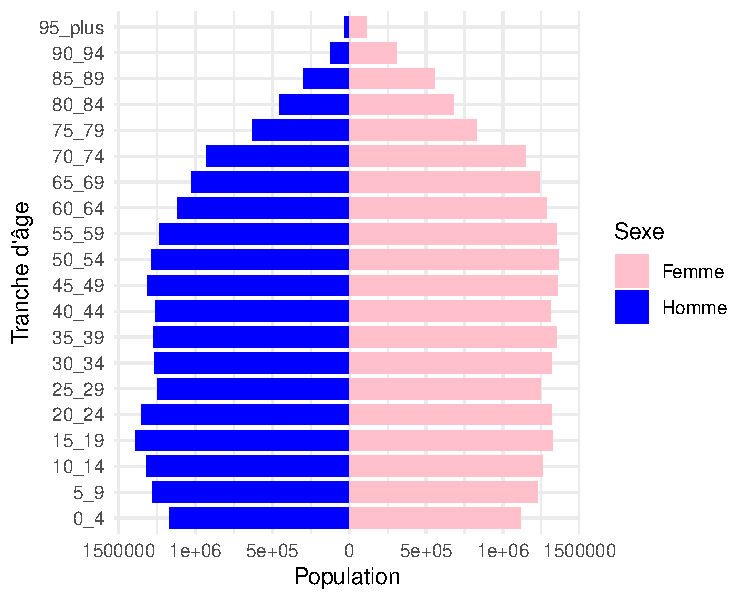
\includegraphics{rapport_intermediaire_files/figure-latex/unnamed-chunk-16-1} 

}

\caption{Pyramide des âges}\label{fig:unnamed-chunk-16}
\end{figure}

\hypertarget{taux-de-natalituxe9-et-taux-de-mortalituxe9}{%
\subsubsection{Taux de natalité et taux de
mortalité}\label{taux-de-natalituxe9-et-taux-de-mortalituxe9}}

Dans les commmunes étudiées, le taux de natalité et de mortalité sont un
peu élevées avec la plupart des taux variant entre 5 et 15 pour 1000 en
ce qui concerne la natalité et 0 et 20 pour 1000 pour la mortalité. On
remarque une corrélation négative entre ces deux taux. Néanmoins cette
corrélation n'a à priori aucun sens. Par ailleurs, l'observation des
distributions permet de constater que la natalité est de façon générale
élevée par rapport à la mortalité dans les communes étudiées.

\begin{figure}

{\centering 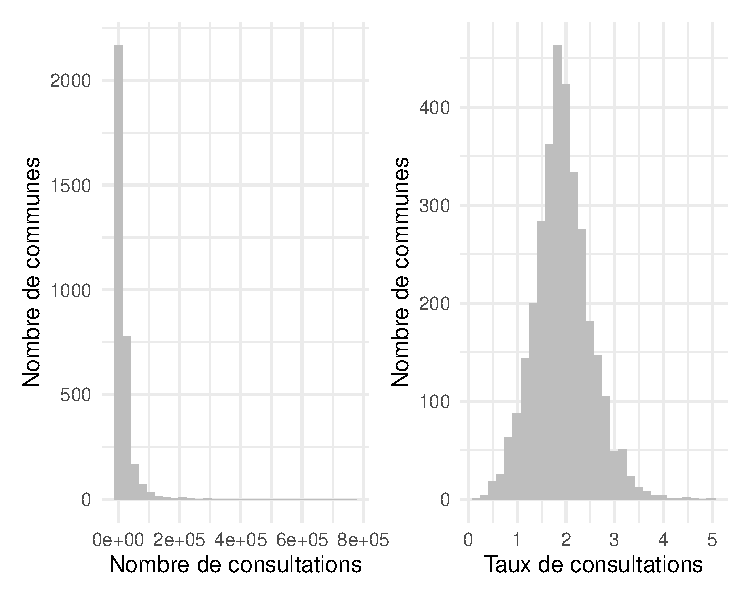
\includegraphics{rapport_intermediaire_files/figure-latex/unnamed-chunk-17-1} 

}

\caption{Taux de Natalité et Taux de Mortalité}\label{fig:unnamed-chunk-17}
\end{figure}

En vue de mieux voir peut être l'effet de la mortalité sur la natalité,
nous allons nous intéresser alors à une analyse de la corrélation entre
les deux taux par groupe d'age. Nous avons considérer les groupes d'âge
suivants : 0-24, 25-44, 45-60, 60 et plus en fonction des variables
disponibles et ausi à partir de l'information sur l'âge des femmes en
âge de procréer qui est de l'ordre de 25-45 et des personnes âgées dont
l'âge est de plus 60 ans. Ne disposant pas du taux de mortalité dans
chaque groupe, alors nous avons dans notre analyse opté plutôt pour le
pourcentage des femmes de chaque groupe en partant du principe que la
natalité est très souvent liée aux femmes et du fait que nous pouvons
analyser une diminution du pourcentage comme étant dû à une mortalité.
Ainsi sur la base de cette nouvelle hypothèse, voici nos nouveaux
résultats.

\begin{figure}

{\centering 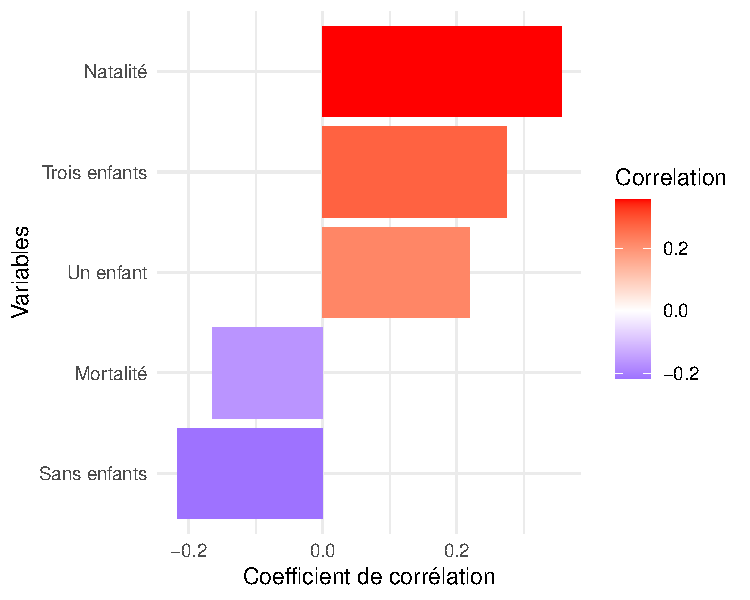
\includegraphics{rapport_intermediaire_files/figure-latex/unnamed-chunk-18-1} 

}

\caption{Taux de Natalité et Pourcentage des femmes dans chaque groupe}\label{fig:unnamed-chunk-18}
\end{figure}

Les résultats nous montrent un lien croissant pour les tranches d'âge
0-24 et 25-45 ans montrant ainsi que dans ces tranches d'âge si le
pourcentage des femmes diminuent (quer l'on pourrait assimiler à une
mort des femmes) alors le taux de natalité diminue. Par ailleurs ceux de
la tranche 45-60 semble n'avoir aucun lien sur le taux de natalité.
Enfin il a été constaté un lien négatif pour la tranche d'âge 60 ans et
plus.

\hypertarget{taux-et-nombre-de-visites}{%
\subsection{Taux et nombre de visites}\label{taux-et-nombre-de-visites}}

(Insérer les cartes à ce niveau : Richard doit refaire les cartes et les
insérer)

L'analyse des statistiques descriptives sur le nombre de visites
annuelles de médecin généraliste entre 2018 et 2022 révèle une
distribution fortement asymétrique à droite, avec une grande dispersion
des données. La moyenne de 19130 visites, nettement supérieure à la
médiane de 9127, indique la présence de valeurs extrêmes tirant la
distribution vers le haut. Cette asymétrie est confirmée par l'écart
considérable entre le minimum de 1037 et le maximum de 765833 visites
par an.

\begin{figure}

{\centering 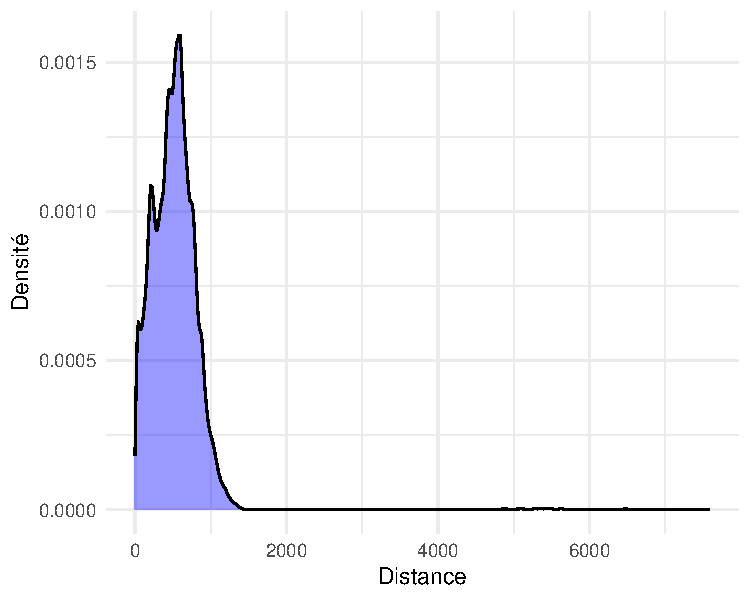
\includegraphics{rapport_intermediaire_files/figure-latex/unnamed-chunk-19-1} 

}

\caption{Distributiion du nombre et du taux de visites}\label{fig:unnamed-chunk-19}
\end{figure}

La moitié des médecins généralistes effectuent entre 5993 et 17290
consultations annuellement, ce qui suggère une variabilité importante
dans la charge de travail. La médiane de 9127 consultations par an,
équivalant à environ 25 consultations par jour ouvrable, semble plus
représentative de l'activité typique d'un médecin généraliste que la
moyenne influencée par les valeurs extrêmes. Ces statistiques mettent en
lumière la diversité des pratiques et des charges de travail parmi les
médecins généralistes, avec potentiellement quelques cas atypiques
présentant un volume de consultations exceptionnellement élevé.

Le nombre de visites pouvant potentiellement être influencé par la
taille de la commune et donc par sa population, nous avons éliminer cet
effet en calculant le taux de consultations qui n'est autre que le
nombre de consultations moyennes par personnes.

\begin{table}[H]
\centering
\caption{\label{tab:unnamed-chunk-20}Résumé statistique du nombre de visites}
\centering
\begin{tabular}[t]{rrrrrr}
\toprule
Min. & 1st Qu. & Median & Mean & 3rd Qu. & Max.\\
\midrule
\cellcolor{gray!10}{1037} & \cellcolor{gray!10}{5993} & \cellcolor{gray!10}{9127} & \cellcolor{gray!10}{19129.63} & \cellcolor{gray!10}{17290} & \cellcolor{gray!10}{765833}\\
\bottomrule
\end{tabular}
\end{table}

\hypertarget{taux-de-visites-et-quelques-variables-duxe9mographiques-et-socio-uxe9conomiques}{%
\subsection{Taux de visites et quelques variables démographiques et
socio-économiques}\label{taux-de-visites-et-quelques-variables-duxe9mographiques-et-socio-uxe9conomiques}}

Nous allons ici, voir s'il y a un lien à priori entre le taux de visites
et certaines de nos variables explicatives. Ainsi, nous avons d'abord
réalisé une analyse descriptive bivariée puis nous avons calculé la
corrélation de Pearson pour évaluer le lien linéaire entre le taux de
consulation et des variables telles que la population totale, la part
des personnes agées (75 ans et plus), la part de quelques CSP (ouvriers
et retraités).

\hypertarget{taux-de-visites-et-population-totale}{%
\subsubsection{Taux de visites et population
totale}\label{taux-de-visites-et-population-totale}}

En divisant les communes en trois groupes égaux (ou presque égaux) en
fonction de la population totale, il ressort un lien clair entre la
taille des communes françaises et le taux de visites médicales, mettant
en évidence une tendance où les grandes communes (\textgreater{} 8974
habitants) affichent un taux moyen de visites supérieur (1,526810) par
rapport aux communes moyennes (1,456356) et petites (1,383861). Cette
observation suggère que l'accès facilité aux infrastructures médicales
dans les zones urbaines contribue à une utilisation accrue des services
de santé. En revanche, les petites communes, probablement plus isolées
et moins dotées en praticiens, semblent rencontrer des barrières
structurelles limitant la fréquence des visites.

\begin{table}[H]
\centering
\caption{\label{tab:unnamed-chunk-21}Taux de visites selon la taille de la commune}
\centering
\begin{tabular}[t]{lr}
\toprule
taille\_commune & Taux de consulations\\
\midrule
\cellcolor{gray!10}{Grande (> 8974)} & \cellcolor{gray!10}{1.526810}\\
Moyenne (4849 - 8974) & 1.456356\\
\cellcolor{gray!10}{Petite (<= 4848)} & \cellcolor{gray!10}{1.383861}\\
\bottomrule
\end{tabular}
\end{table}

\hypertarget{taux-de-visites-et-population-uxe2guxe9e}{%
\subsubsection{Taux de visites et population
âgée}\label{taux-de-visites-et-population-uxe2guxe9e}}

L'analyse met en évidence que les communes françaises avec une
population âgée significative (population âgée de 75 ans et plus est
supérieure à la médiane soit plus de 670 habitants âgés de 75 ans et
plus) présentent un taux moyen de visistes inférieur (1,410213) comparé
aux communes où la population âgée est moindre (1,501111). Cette
observation peut refléter des défis spécifiques aux populations plus
âgées, tels que des obstacles physiques ou logistiques pour accéder aux
soins médicaux, ou encore une moindre propension à consulter
régulièrement en raison d'habitudes ou de conditions de santé
chroniques. Ces résultats soulignent un paradoxe apparent, car les
besoins en soins médicaux des personnes âgées sont en général plus
importants, ce qui pourrait indiquer une inadéquation entre l'offre
médicale et les besoins spécifiques de cette tranche d'âge. Cela met en
lumière un enjeu crucial pour les politiques de santé visant à améliorer
l'accès et l'utilisation des services médicaux pour les populations
vieillissantes.

\begin{table}[H]
\centering
\caption{\label{tab:unnamed-chunk-22}Taux de visites selon la population âgée}
\centering
\begin{tabular}[t]{lr}
\toprule
population\_agee\_importante & consultations\_moyennes\\
\midrule
\cellcolor{gray!10}{Non (<= 670)} & \cellcolor{gray!10}{1.501111}\\
Oui (> 670) & 1.410213\\
\bottomrule
\end{tabular}
\end{table}

\hypertarget{taux-de-visites-et-csp}{%
\subsubsection{Taux de visites et CSP}\label{taux-de-visites-et-csp}}

Aucune catégorie ne semble montrer une relation linéaire évidente avec
le taux de visites. Par ailleurs, pour toutes les catégories
socio-professionnelles, la majorité des communes se situent dans une
plage de proportions faibles, ce qui limite la variabilité observable
dans les relations. Une analyse statistique supplémentaire, comme le
calcul de corrélations, serait nécessaire pour confirmer ou infirmer les
relations observées visuellement.

\begin{figure}

{\centering 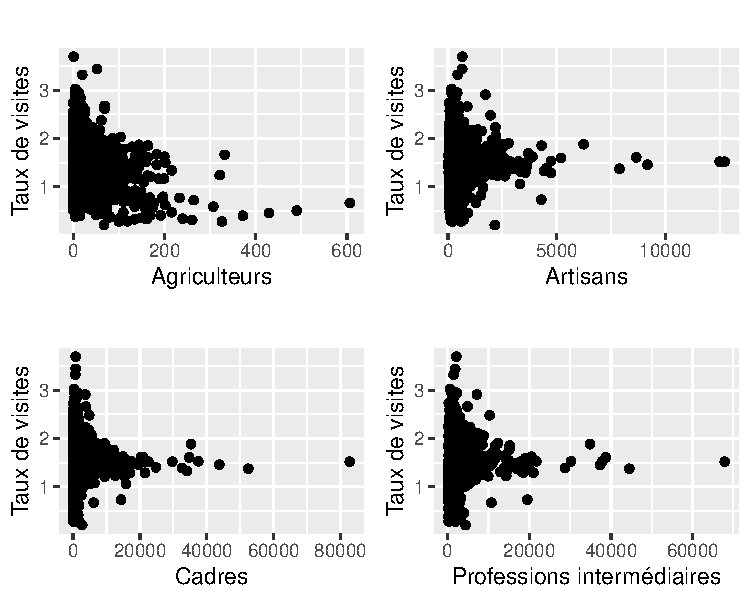
\includegraphics{rapport_intermediaire_files/figure-latex/unnamed-chunk-23-1} 

}

\caption{Relations entre le taux de visites et certaines catégories socioprofessionnelles (variables standarisées)}\label{fig:unnamed-chunk-23}
\end{figure}

\hypertarget{trouver-un-titre-pour-cette-section-et-analyser-alex}{%
\subsubsection{(Trouver un titre pour cette section et analyser :
Alex)}\label{trouver-un-titre-pour-cette-section-et-analyser-alex}}

\begin{figure}

{\centering 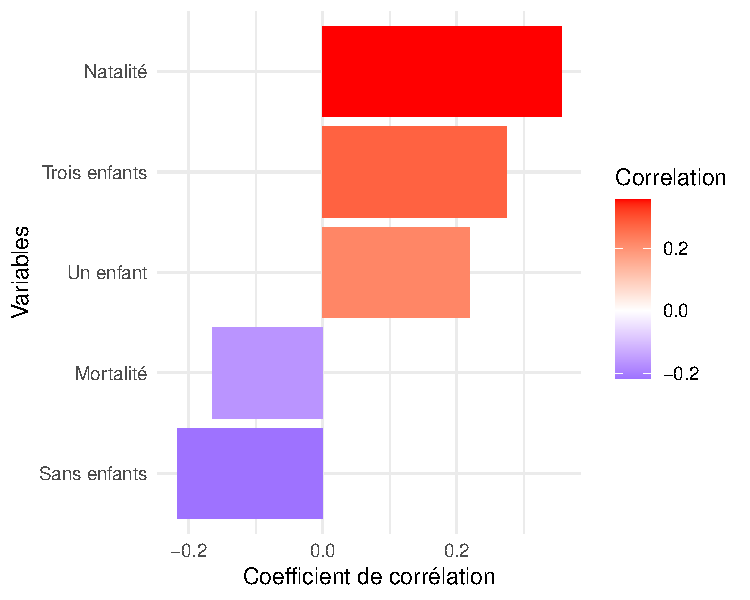
\includegraphics{rapport_intermediaire_files/figure-latex/unnamed-chunk-24-1} 

}

\caption{Corrélations entre le nombre de visite et quelques variables}\label{fig:unnamed-chunk-24}
\end{figure}

\hypertarget{analyse-spatiale}{%
\subsection{Analyse spatiale}\label{analyse-spatiale}}

Après une analyse de nos données en ne tenant pas compte de l'effet
spatial, nous allons à présent poursuivre avec une analyse qui tient
compte de celui-ci. Nous allons ici faire une analyse basée sur le
diagramme de Moran. Ainsi d'après les explications données au niveau de
la partie méthodologie, nous aurons les 4 quadrants suivants.

\begin{itemize}
\tightlist
\item
  \textbf{Quadrant 1 (haut à droite)} : Les zones avec un taux de
  consultations plus élevé que la moyenne, entourées de zones présentant
  également un taux de consultations élevé (autocorrélation spatiale
  positive, structure \textbf{high-high}).
\item
  \textbf{Quadrant 3 (bas à gauche)} : Les zones avec un taux de
  consultations plus faible que la moyenne, entourées de zones
  présentant un taux de consultations également faible (autocorrélation
  spatiale positive, structure \textbf{low-low}).
\item
  \textbf{Quadrant 2 (bas à droite)} : Les zones avec un taux de
  consultations plus élevé que la moyenne, mais entourées de zones
  présentant un taux de consultations plus faible (autocorrélation
  spatiale négative, structure \textbf{high-low}).
\item
  \textbf{Quadrant 4 (haut à gauche)} : Les zones avec un taux de
  consultations plus faible que la moyenne, mais entourées de zones avec
  un taux de consultations plus élevé (autocorrélation spatiale
  négative, structure \textbf{low-high}).
\end{itemize}

Vu le nombre de nos communes, la mise sur le graphique des noms de
toutes les communes allait être compliquée. Pour cela, nous avons choisi
au hasard 4 communes par cadrant. Ainsi, Ce diagramme de Moran illustre
la corrélation spatiale des taux de consultation par commune et ceux des
communes voisines. La tendance générale, représentée par la droite de
régression rouge, montre une relation positive entre ces taux,
confirmant ainsi une autocorrélation spatiale. Autrement dit, les
communes ayant un taux élevé de consultations ont tendance à être
entourées par d'autres communes avec un taux similaire, et inversement.

Dans le quadrant HH (Haut-Haut), représenté en rouge, on retrouve des
communes comme Saint-Saulve, Le Bouscat et Bruay-la-Buissière. Celles-ci
affichent un taux de consultations élevé et sont entourées par des
communes présentant également des taux élevés. Cela indique une
concentration géographique des consultations médicales, qui peut
s'expliquer par une offre de soins plus développée ou une demande locale
particulièrement forte.

Le quadrant HL (Haut-Bas), en violet, comprend des communes comme
Saint-Jacques-de-la-Lande et Le Portel. Ces communes ont un taux élevé
de consultations, mais sont entourées de communes où les taux sont plus
faibles. Ce contraste peut suggérer que ces villes disposent d'une offre
de soins plus attractive que leurs voisines, attirant ainsi des patients
des alentours.

À l'inverse, dans le quadrant LH (Bas-Haut), en vert, on trouve des
communes comme Aix-en-Provence, Ribécourt-Dreslincourt et L'Isle-Adam.
Ces communes affichent un faible taux de consultations, tandis que leurs
voisines présentent des taux plus élevés. Ce phénomène peut s'expliquer
par le fait que les habitants de ces villes se rendent dans les communes
avoisinantes pour leurs consultations, soit en raison d'un manque
d'infrastructures médicales locales, soit par préférence pour des
services situés ailleurs.

Enfin, le quadrant LL (Bas-Bas), en orange, inclut des communes comme
Saint-Jean-le-Blanc, Romorantin-Lanthenay et Le Breuil. Ces villes ont
un faible taux de consultations et sont entourées de communes où les
taux sont également bas. Cela peut indiquer une accessibilité réduite
aux soins de santé, une moindre densité médicale, ou encore une faible
demande locale pour des consultations.

En résumé, cette analyse met en évidence des disparités territoriales
dans la répartition des consultations médicales. Certaines communes
concentrent les services et attirent les patients des alentours, tandis
que d'autres souffrent d'un accès limité aux soins, renforçant ainsi les
inégalités spatiales en matière de santé.

\begin{figure}

{\centering 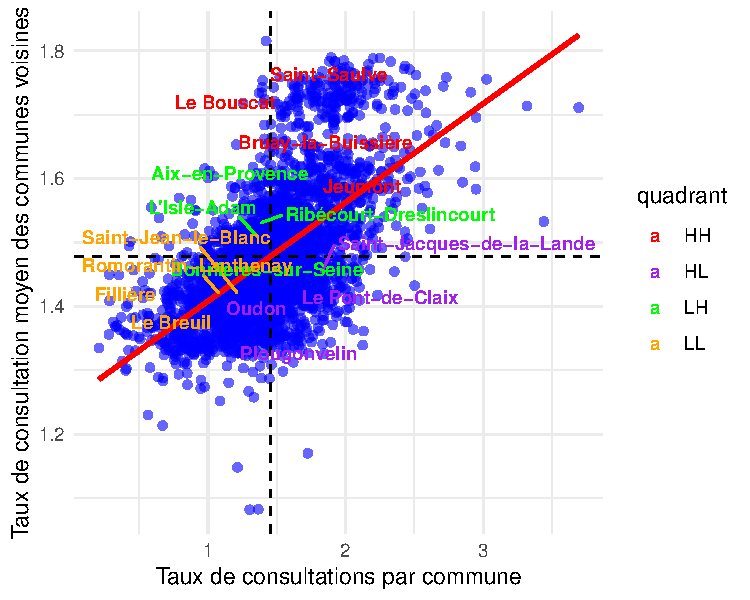
\includegraphics{rapport_intermediaire_files/figure-latex/unnamed-chunk-32-1} 

}

\caption{Moran Plot avec visibilités de quelques communes}\label{fig:unnamed-chunk-32}
\end{figure}

\hypertarget{autocoruxe9lation-locale}{%
\subsubsection{Autocorélation locale}\label{autocoruxe9lation-locale}}

En se basant sur l'analyse par cluster fourni pour le LISA (local
Indicator or Spatial Association), nous pouvons remarquer que le cluster
HH est celui regroupant le plus de communes suivi du cluster LH. Ceci
dit une grande partie des communes ont des taux élevées et entourées par
des communes avec des taux élevés ou encore des taux bas et entourées
par des communes ayant des taux élevés.

\begin{figure}

{\centering 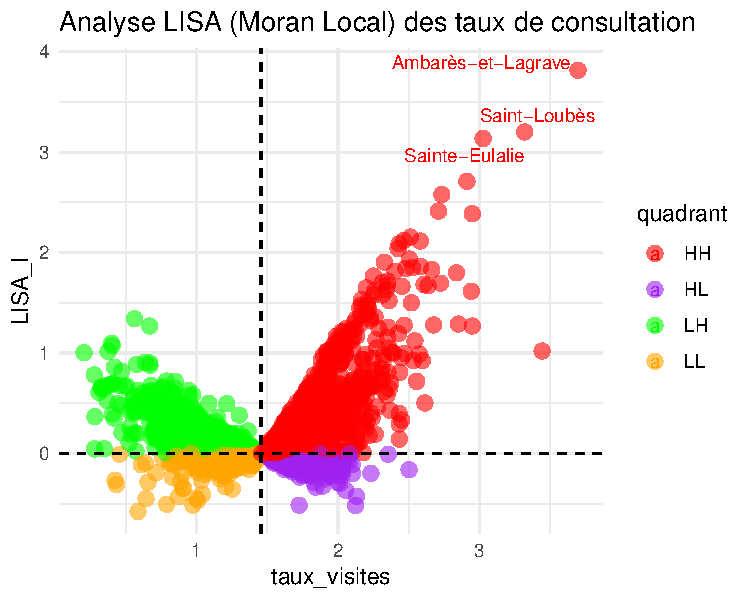
\includegraphics{rapport_intermediaire_files/figure-latex/unnamed-chunk-33-1} 

}

\caption{Clusters sur la base du LISA}\label{fig:unnamed-chunk-33}
\end{figure}

\hypertarget{annexes}{%
\section{Annexes}\label{annexes}}

\begin{figure}
    \centering
    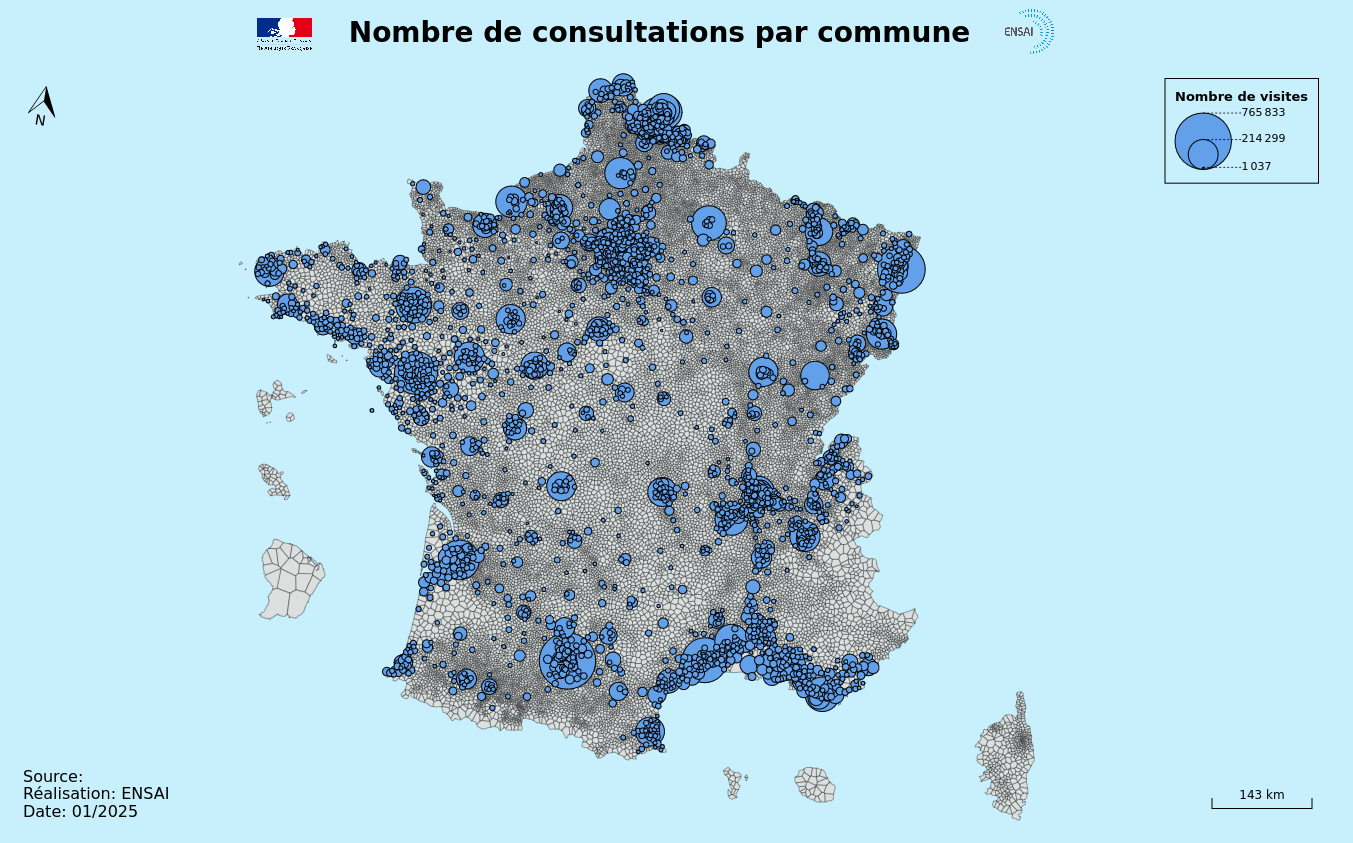
\includegraphics[width=1\linewidth]{../cartes/nombre_de_consulatations}
    \caption{Carte du nombre de consultations par commune}
    \label{fig:figure}
\end{figure}
\begin{figure}
    \centering
    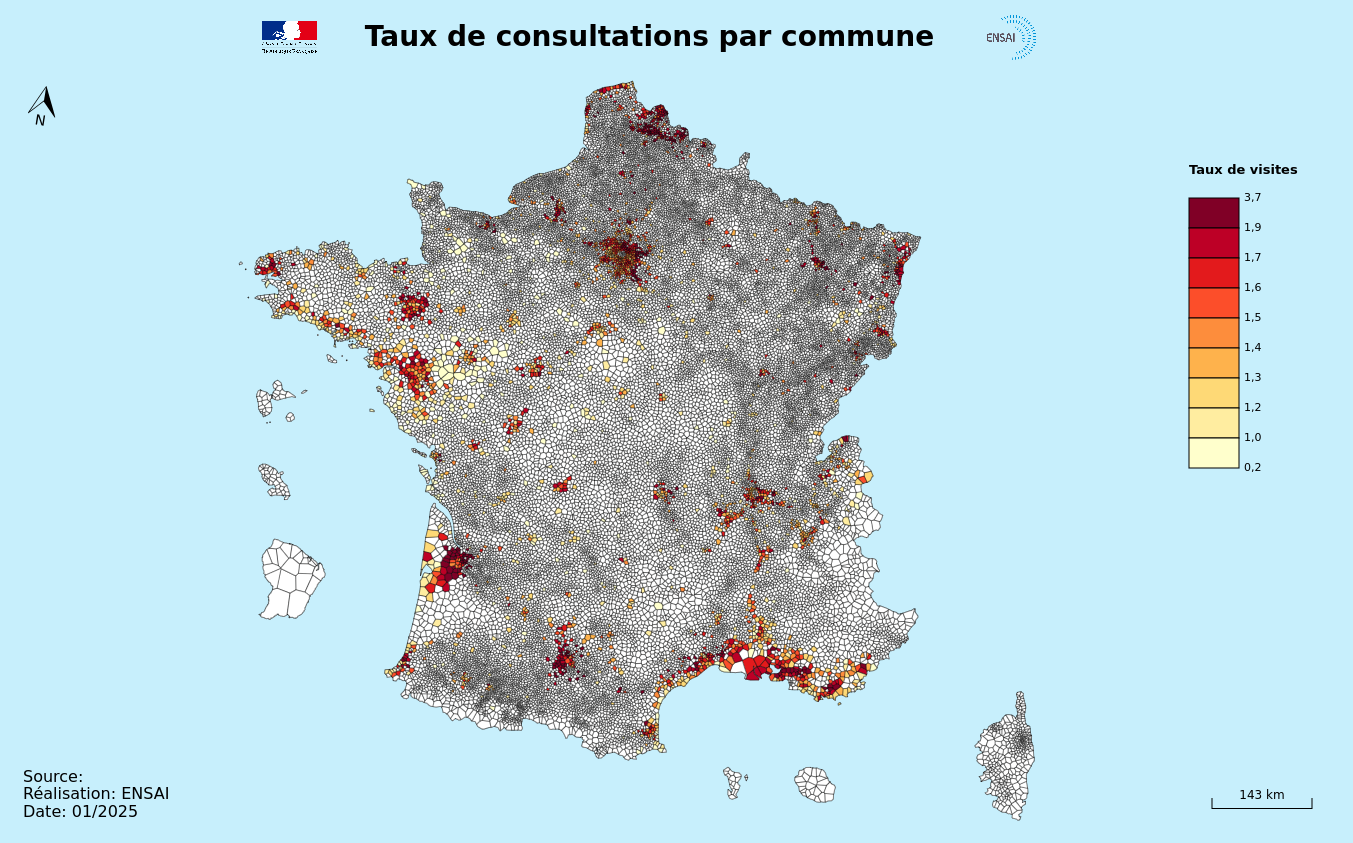
\includegraphics[width=1\linewidth]{../cartes/taux_de_consultations}
    \caption{Carte du taux de consultations par commune}
    \label{fig:figure}
\end{figure}
\begin{figure}
    \centering
    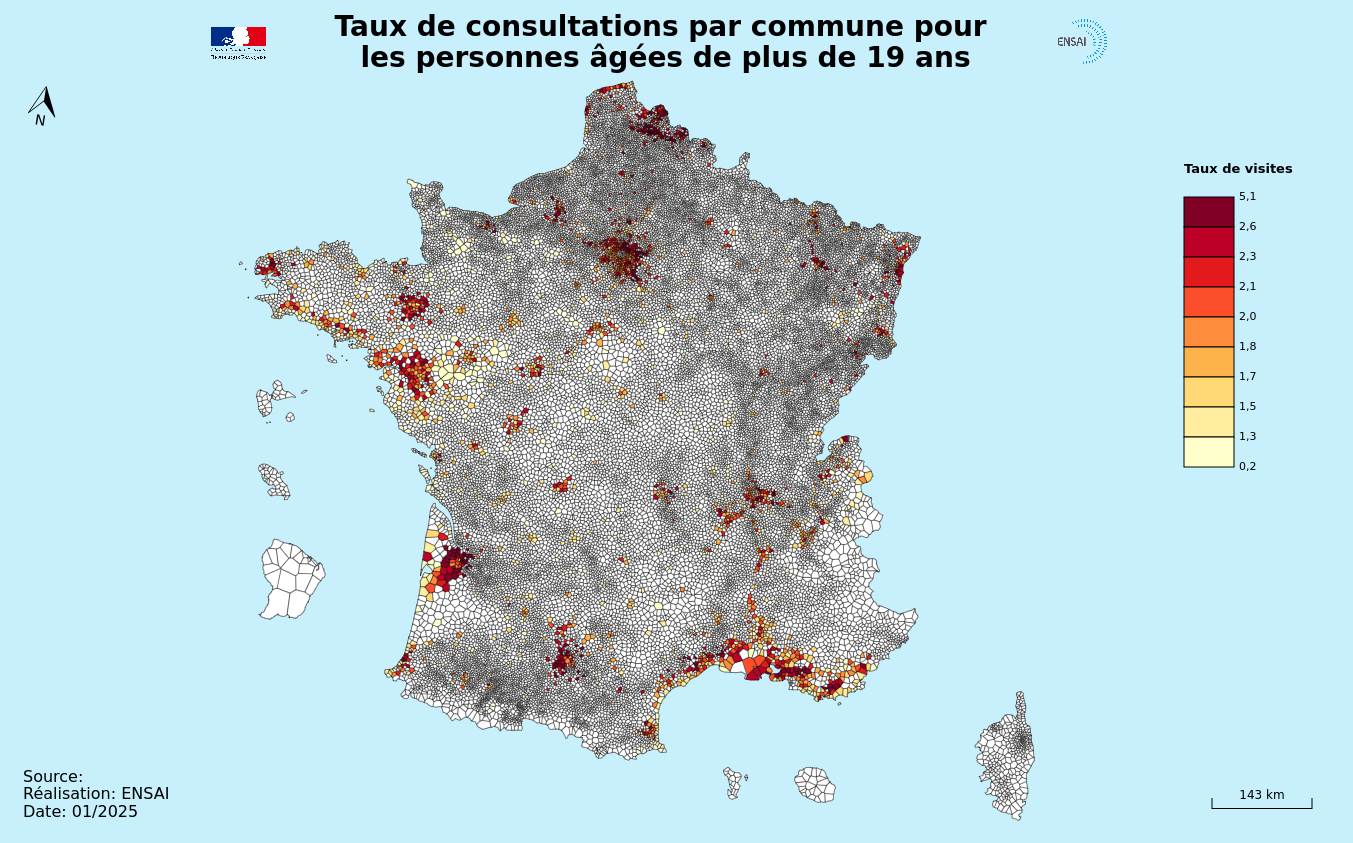
\includegraphics[width=1\linewidth]{../cartes/taux_de_consultations_plus_19_ans}
    \caption{Carte du taux de consultations par commune pour les plus de 19 ans}
    \label{fig:figure}
\end{figure}

\hypertarget{refs}{}
\begin{CSLReferences}{1}{0}
\leavevmode\vadjust pre{\hypertarget{ref-bfmtv2024}{}}%
BFMTV. 2024. {«~Généraliste, dermatologue, pédiatre : quel est le délai
pour obtenir un rendez-vous chez le médecin en 2024 ?~»}
\url{https://www.bfmtv.com/tech/vie-numerique/sur-doctolib-la-moitie-des-consultations-de-generalistes-sont-obtenues-en-moins-de-3-jours_AD-202404230604.html}.

\leavevmode\vadjust pre{\hypertarget{ref-statcan2022}{}}%
Canada, Statistique. 2022. {«~Fréquence des consultations médicales et
facteurs sociodémographiques~»}. \url{https://www150.statcan.gc.ca}.

\leavevmode\vadjust pre{\hypertarget{ref-egora2023}{}}%
Egora. 2023. {«~Hôpital : la part d'ambulatoire augmente de 6,5 \% , les
séjours diminuent~»}.
\url{https://www.egora.fr/actus-pro/hopitaux/hopital-la-part-dambulatoire-augmente-de-65-les-sejours-diminuent}.

\leavevmode\vadjust pre{\hypertarget{ref-irdes2020}{}}%
Irdes. 2020. {«~Inégalités spatiales d'accessibilité aux soins
médicaux~»}. \url{https://www.irdes.fr}.

\end{CSLReferences}

\end{document}
